\begin{frame}
	\frametitle{Demo}

Time for a demo!

\end{frame}

\begin{frame}
	\frametitle{Function identification through fuzzy callgraph matching}

\textbf{Example}: source program compiled for three different machine architectures.

	\begin{figure}[htbp]
		\centering
		\begin{subfigure}[t]{0.32\textwidth}
			\centering
			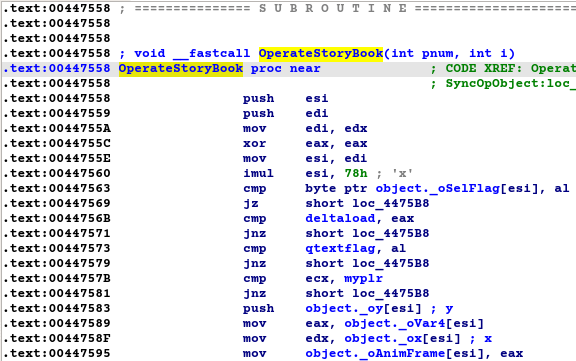
\includegraphics[width=\linewidth,valign=t]{inc/example/x86_zoom.png}
			\caption{x86 assembly.}
		\end{subfigure}
		\hfill
		\begin{subfigure}[t]{0.32\textwidth}
			\centering
			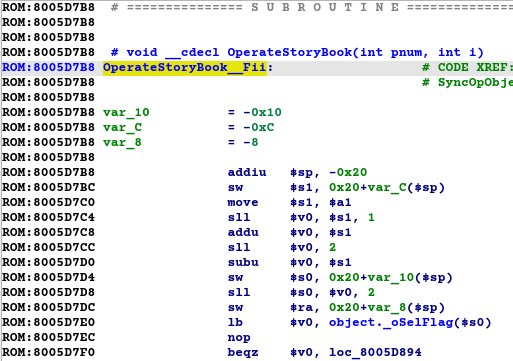
\includegraphics[width=\linewidth,valign=t]{inc/example/mips_zoom.png}
			\caption{MIPS assembly.}
		\end{subfigure}
		\hfill
		\begin{subfigure}[t]{0.32\textwidth}
			\centering
			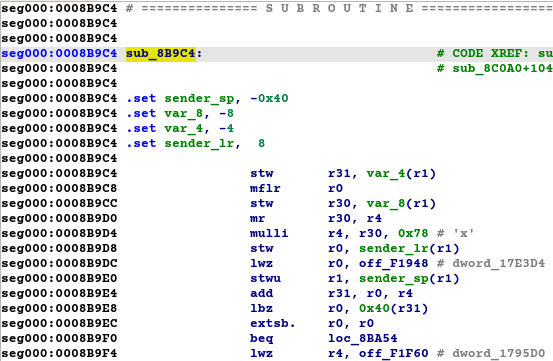
\includegraphics[width=\linewidth,valign=t]{inc/example/ppc_zoom.png}
			\caption{PowerPC assembly.}
		\end{subfigure}
		\caption{Machine code of the same source function in x86 (left), MIPS (middle) and PowerPC (right) assembly.}
	\end{figure}

\end{frame}

\begin{frame}
	\frametitle{Function identification through fuzzy callgraph matching}

	\begin{figure}[htbp]
		%\centering
		\begin{subfigure}{1\textwidth}
			\centering
			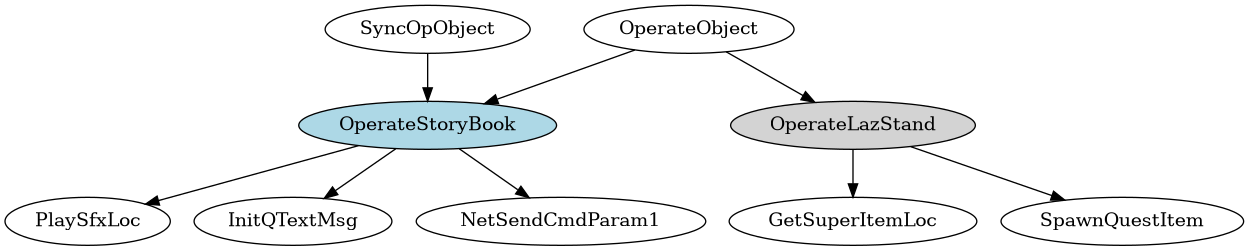
\includegraphics[width=0.65\linewidth]{inc/example/callgraph_x86.png}
			\caption{x86 callgraph.}
		\end{subfigure}
		\begin{subfigure}{1\textwidth}
			\centering
			\vspace*{1em}
			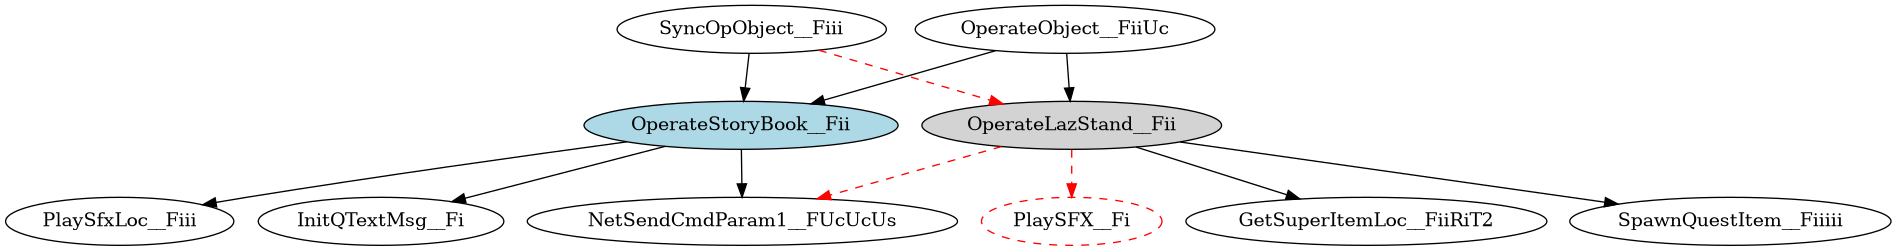
\includegraphics[width=0.9\linewidth]{inc/example/callgraph_mips.png}
			\caption{MIPS callgraph.}
		\end{subfigure}
		\begin{subfigure}{1\textwidth}
			\centering
			\vspace*{1em}
			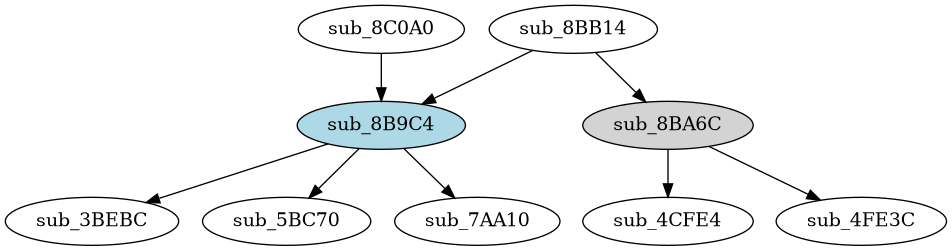
\includegraphics[width=0.5\linewidth]{inc/example/callgraph_ppc_before.png}
			\caption{PowerPC callgraph.}
		\end{subfigure}
		\caption{Corresponding callgraphs for x86 (top), MIPS (middle) and PowerPC (bottom) assembly.}
	\end{figure}

\end{frame}

\begin{frame}
	\frametitle{Function identification through fuzzy callgraph matching}

	\begin{figure}[htbp]
		%\centering
		\begin{subfigure}{1\textwidth}
			\centering
			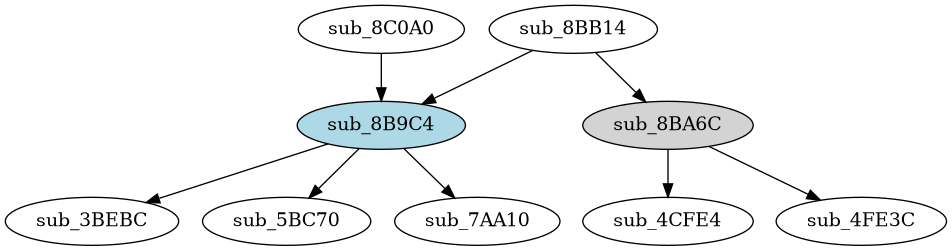
\includegraphics[width=0.7\linewidth]{inc/example/callgraph_ppc_before.png}
			\caption{MIPS callgraph \textit{before} fuzzy callgraph matching.}
		\end{subfigure}
		\begin{subfigure}{1\textwidth}
			\centering
			\vspace*{1em}
			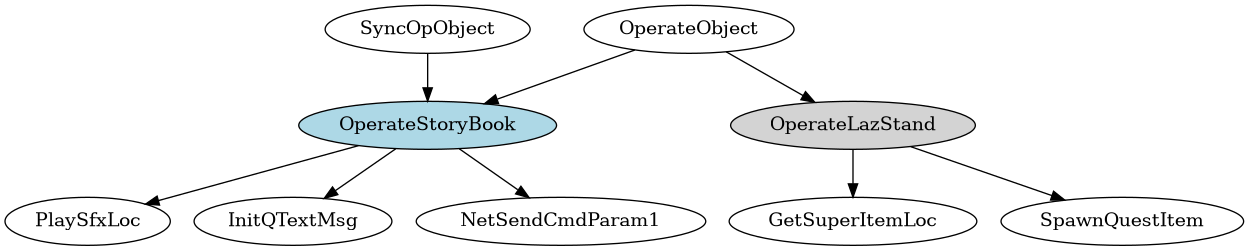
\includegraphics[width=0.9\linewidth]{inc/example/callgraph_ppc_after.png}
			\caption{MIPS callgraph \textit{after} fuzzy callgraph matching.}
		\end{subfigure}
		\caption{Results of fuzzy callgraph matching used to assign names to unknown functions.}
	\end{figure}

\end{frame}

\begin{frame}
	\frametitle{Function identification through fuzzy callgraph matching}

	The example source program has a callgraph with $2551$ verticies and $6400$ edges, illustrating the need for performant algorithms and the benefit of automating function identification.

	\begin{figure}[htbp]
		\centering
		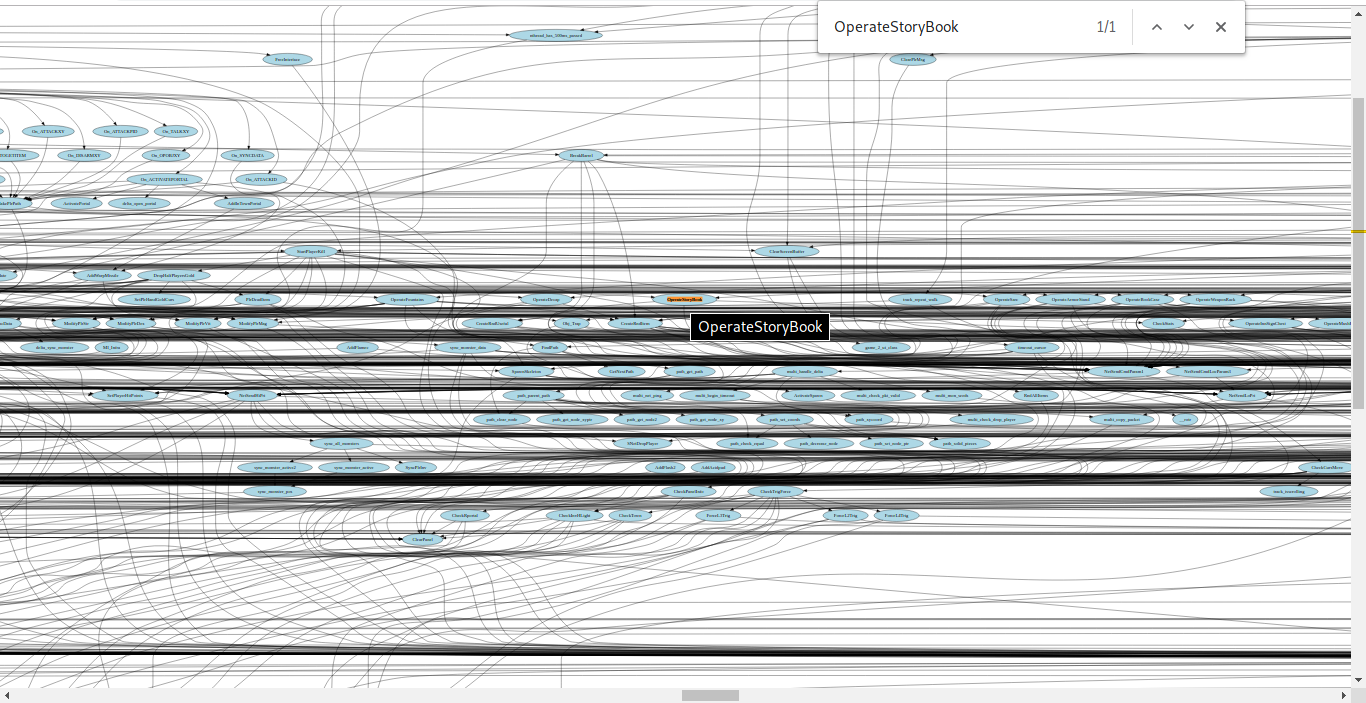
\includegraphics[width=0.85\linewidth]{inc/example/full_callgraph.png}
		\caption{An extract of the callgraph of the source program.}
	\end{figure}
\end{frame}

\begin{frame}
	\frametitle{Function identification through fuzzy callgraph matching}

	For reference, this is the original source code of the C source function \texttt{OperateStoryBook}.

	\begin{figure}[htbp]
		\centering
		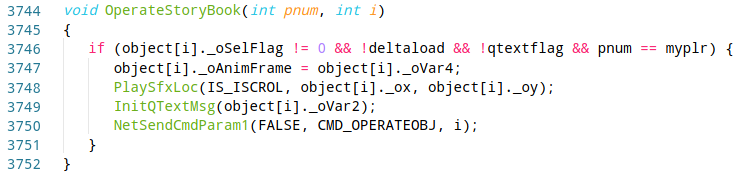
\includegraphics[width=0.8\linewidth]{inc/example/source_func_light.png}
		%\lstinputlisting[language=C, style=c]{inc/example/source_func.c}
		\caption{Original source code of the C source function \texttt{OperateStoryBook}.}
	\end{figure}
\end{frame}
